% !TEX root = ..\proposal.tex

\section{Architecture}
\label{sec:arch}
As can be seen below in Figure \ref{fig:Architecture}, the system architecture consists of 4 main layers; Client, Presentation, Business and Data layers.

\begin{figure}[htp]
    \centering
    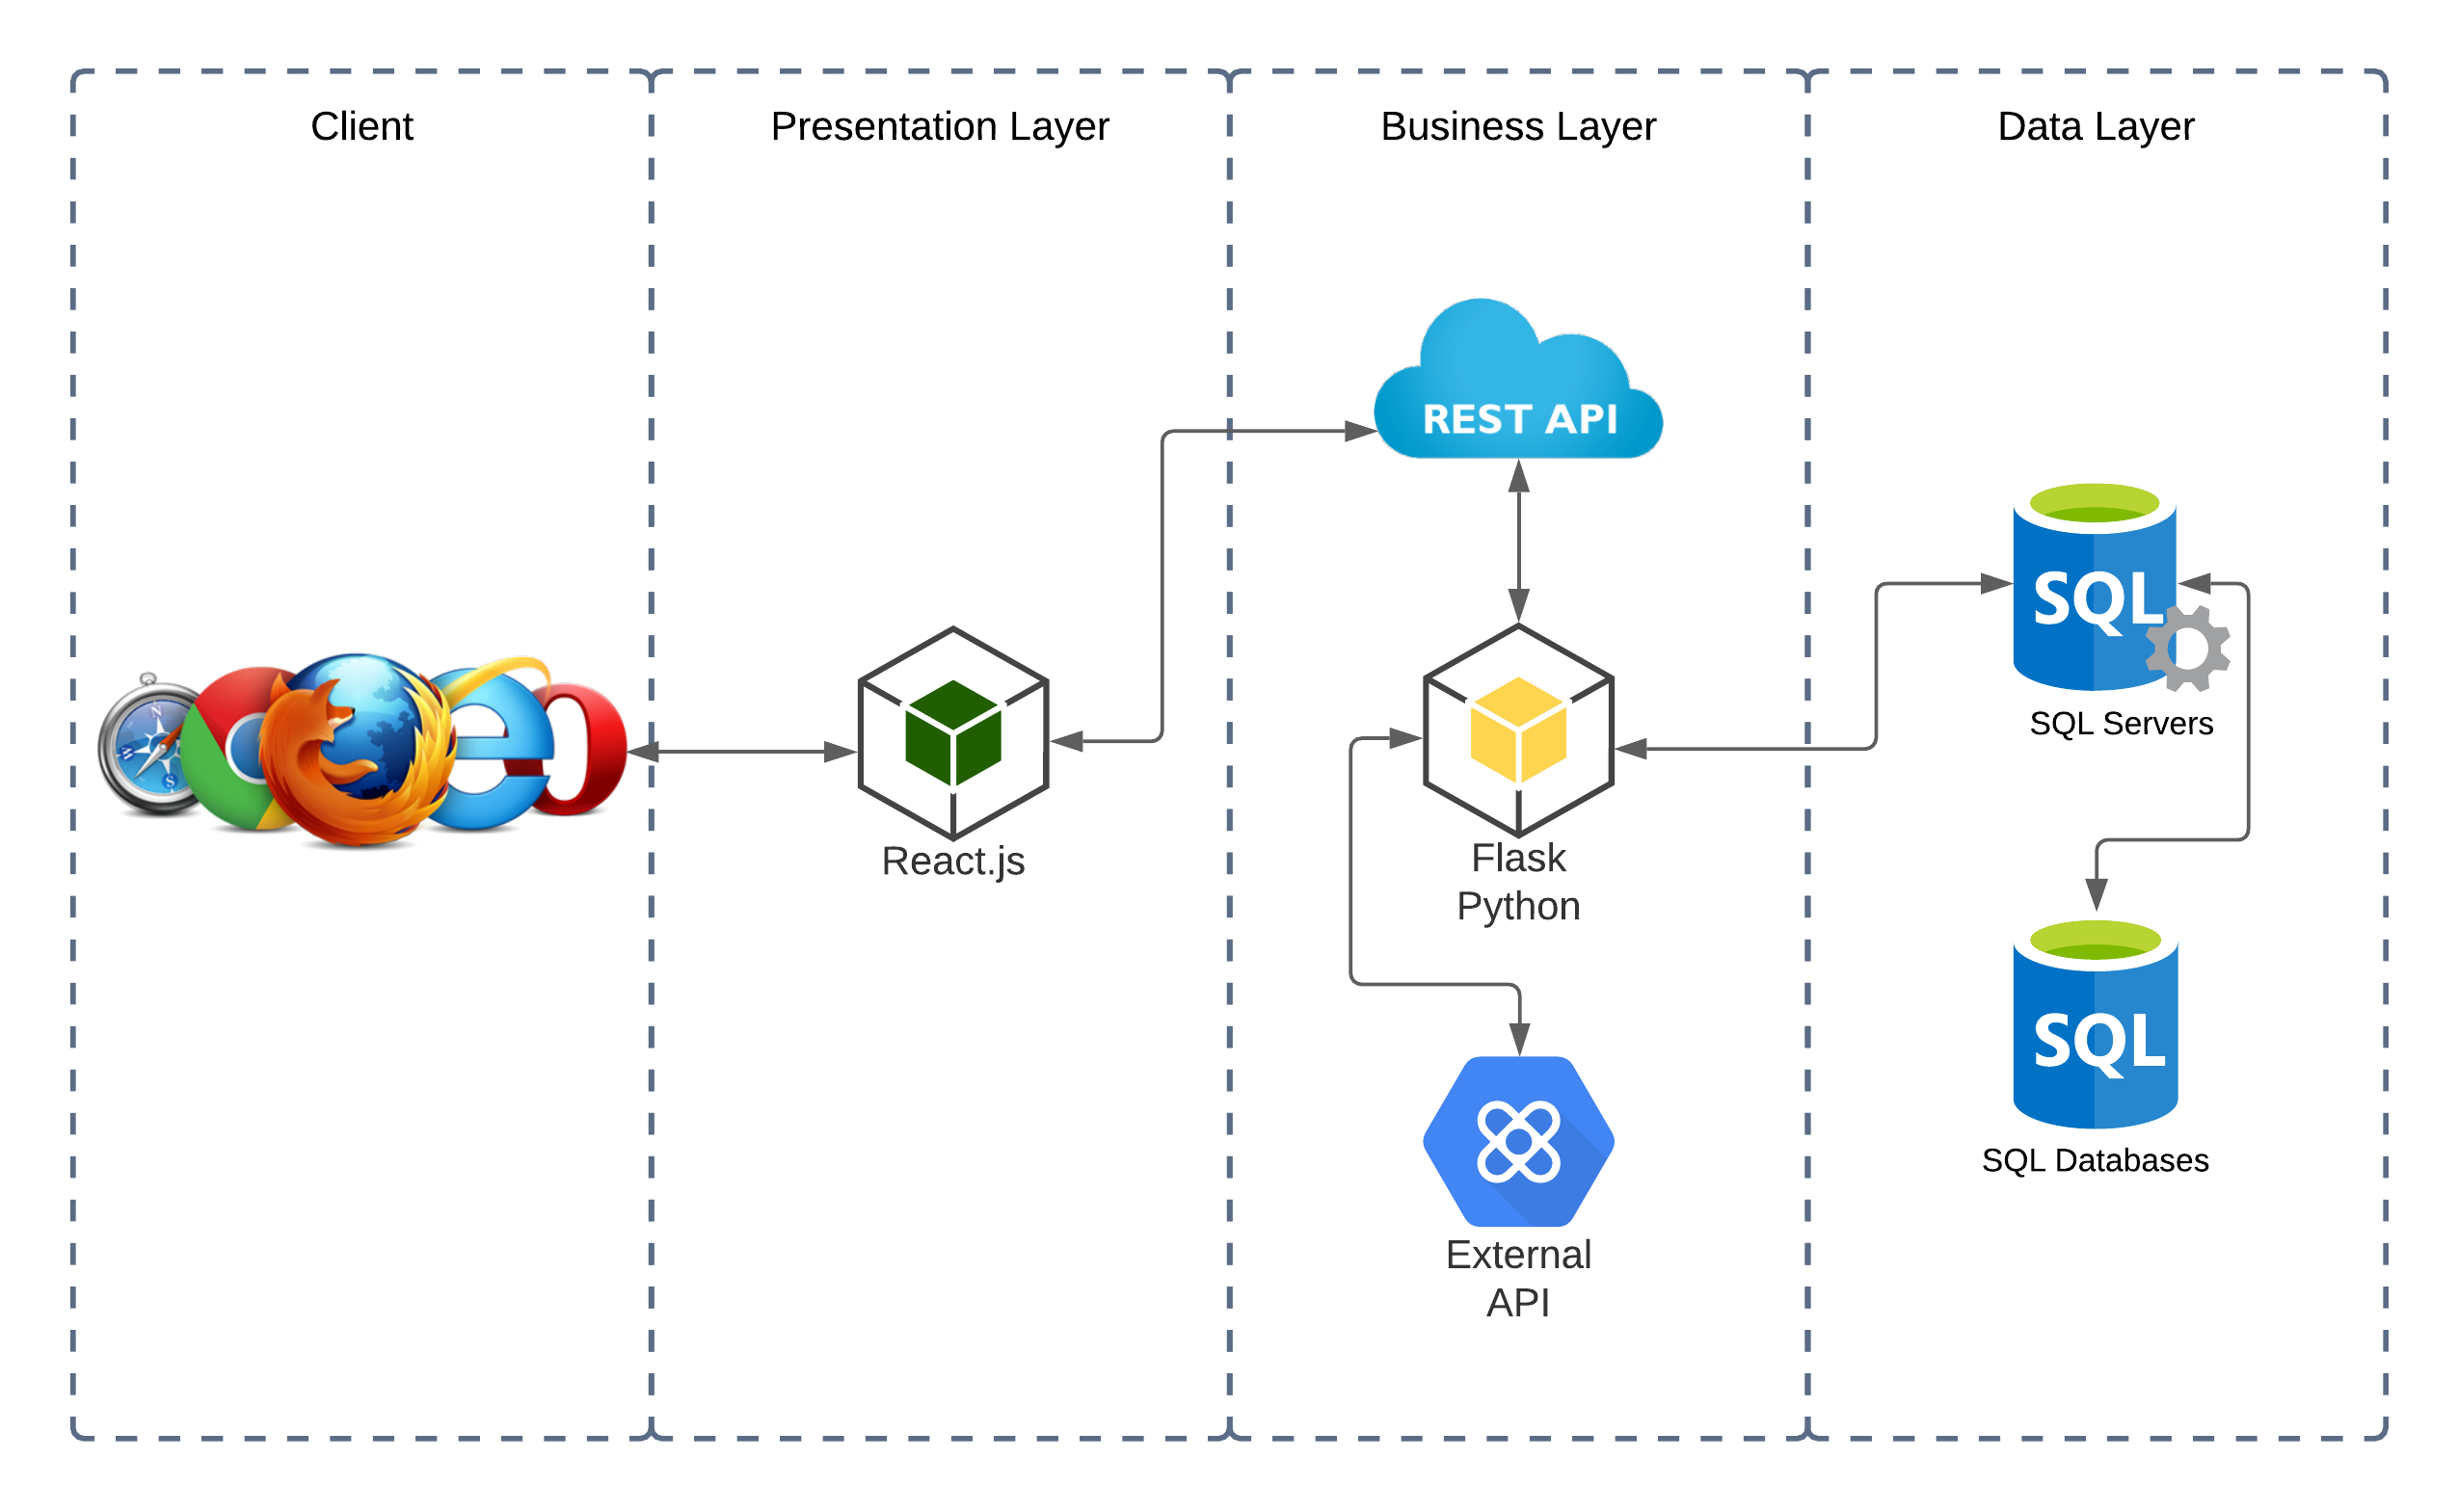
\includegraphics[scale = .7]{./5_architecture/Architecture.png}
    \caption{Simvestr - Layered Architecture Diagram}
    \label{fig:Architecture}
\end{figure}


In the Client and Presentation layers, a user will interact via their browser directly with the client-side rendered ReactJS application. Any requests for data which the application may make will be routed to the exposed REST API endpoints provided by the Business layer. Python with SQLAlchemy is used in the Business layer which interacts with the SQLite database in the Data layer. SQLite is used as the database to store all the data due to its low latency and convenience. 

The decision to use SQLAlchemy is important as it allows separability between the RESTful architecture and the data layer. This enables future scalability as the database technology can be changed without any changes to the interaction between the REST APIs and the database.

Additionally, the back-end python server will query external API endpoints such as those provided by \url{https://finnhub.io/} and \url{https://api.tiingo.com} to gather both relevant historical and current market data. This data will be first processed and standardised by the back-end before being served by the exposed (internal) REST APIs and consumed by the front-end.


The four main services which compose the architecture and their associated technologies are outlined below:
\begin{itemize}[leftmargin=*,topsep=8pt,itemsep=2pt,partopsep=4pt, parsep=2pt]
\item Front-end - \textbf{ReactJS, JS (ES11)}
\item Back-end - \textbf{Python}
\item Internal API - \textbf{Flask RESTx}
\item Database - \textbf{SQLite}
\end{itemize}

\subsection{Front-end}
 The front-end encapsulates the user interface which an end user using the service will interact with; it is inherently the presentational layer in the architecture. The front end will be a single page application built using ReactJS (\url{https://reactjs.org/}); a JavaScript (JS) library which is widely adopted in the industry for building such user interfaces. React allows for the creation and modification of an internal state on the client side, allowing for a responsive, asynchronous interactive experience for the end user. Additionally, we will be using packages/modules within the ReactJS ecosystem to further develop the front end application. Ultimately, ReactJS compiles down the vanilla JS, which can then be build and packaged for deployment.

\subsection{Back-end}
The back-end refers to the serving and processing of exposed APIs that the front-end consumes. The back-end will both serve as an intermediary between the front-end and external APIs as well as handling interactions with the database. This allows for a dynamic experience by those interacting with the front-end, as data is able to be asynchronously populated. Being able to make those requests from the client will remove the need to have to do any of that processing before the page is served to the browser. As such, the back-end serves as a RESTful interface between any external APIs and the front-end application.

The REST APIs will use authorisation tokens to allow a user to access data such as; their profile data; their trading history, portfolio value and trends, their watch list and leader-board ranking. These exposed APIs are easily extensible, allowing the application to grow as required with expanding application complexity.

\subsection{User Interaction}
As can be seen in Figure \ref{fig:Simvestr - User Interaction Diagram} the user will interact directly with the front-end application, which will then send requests to the back-ends exposed RESTful APIs. 

For example, if a user searches for a particular stock to obtain current pricing information, the front-end will take that input, perform a GET request against the back-end, which will send another request to the external API to gather the relevant information for that particular stock. Upon success, the back-end will standardise the response, add any additional required information, and send this payload as a response back to the front-end. The front-end will then asynchronously update and display the results of the search.

\begin{figure}[htp]
    \centering
    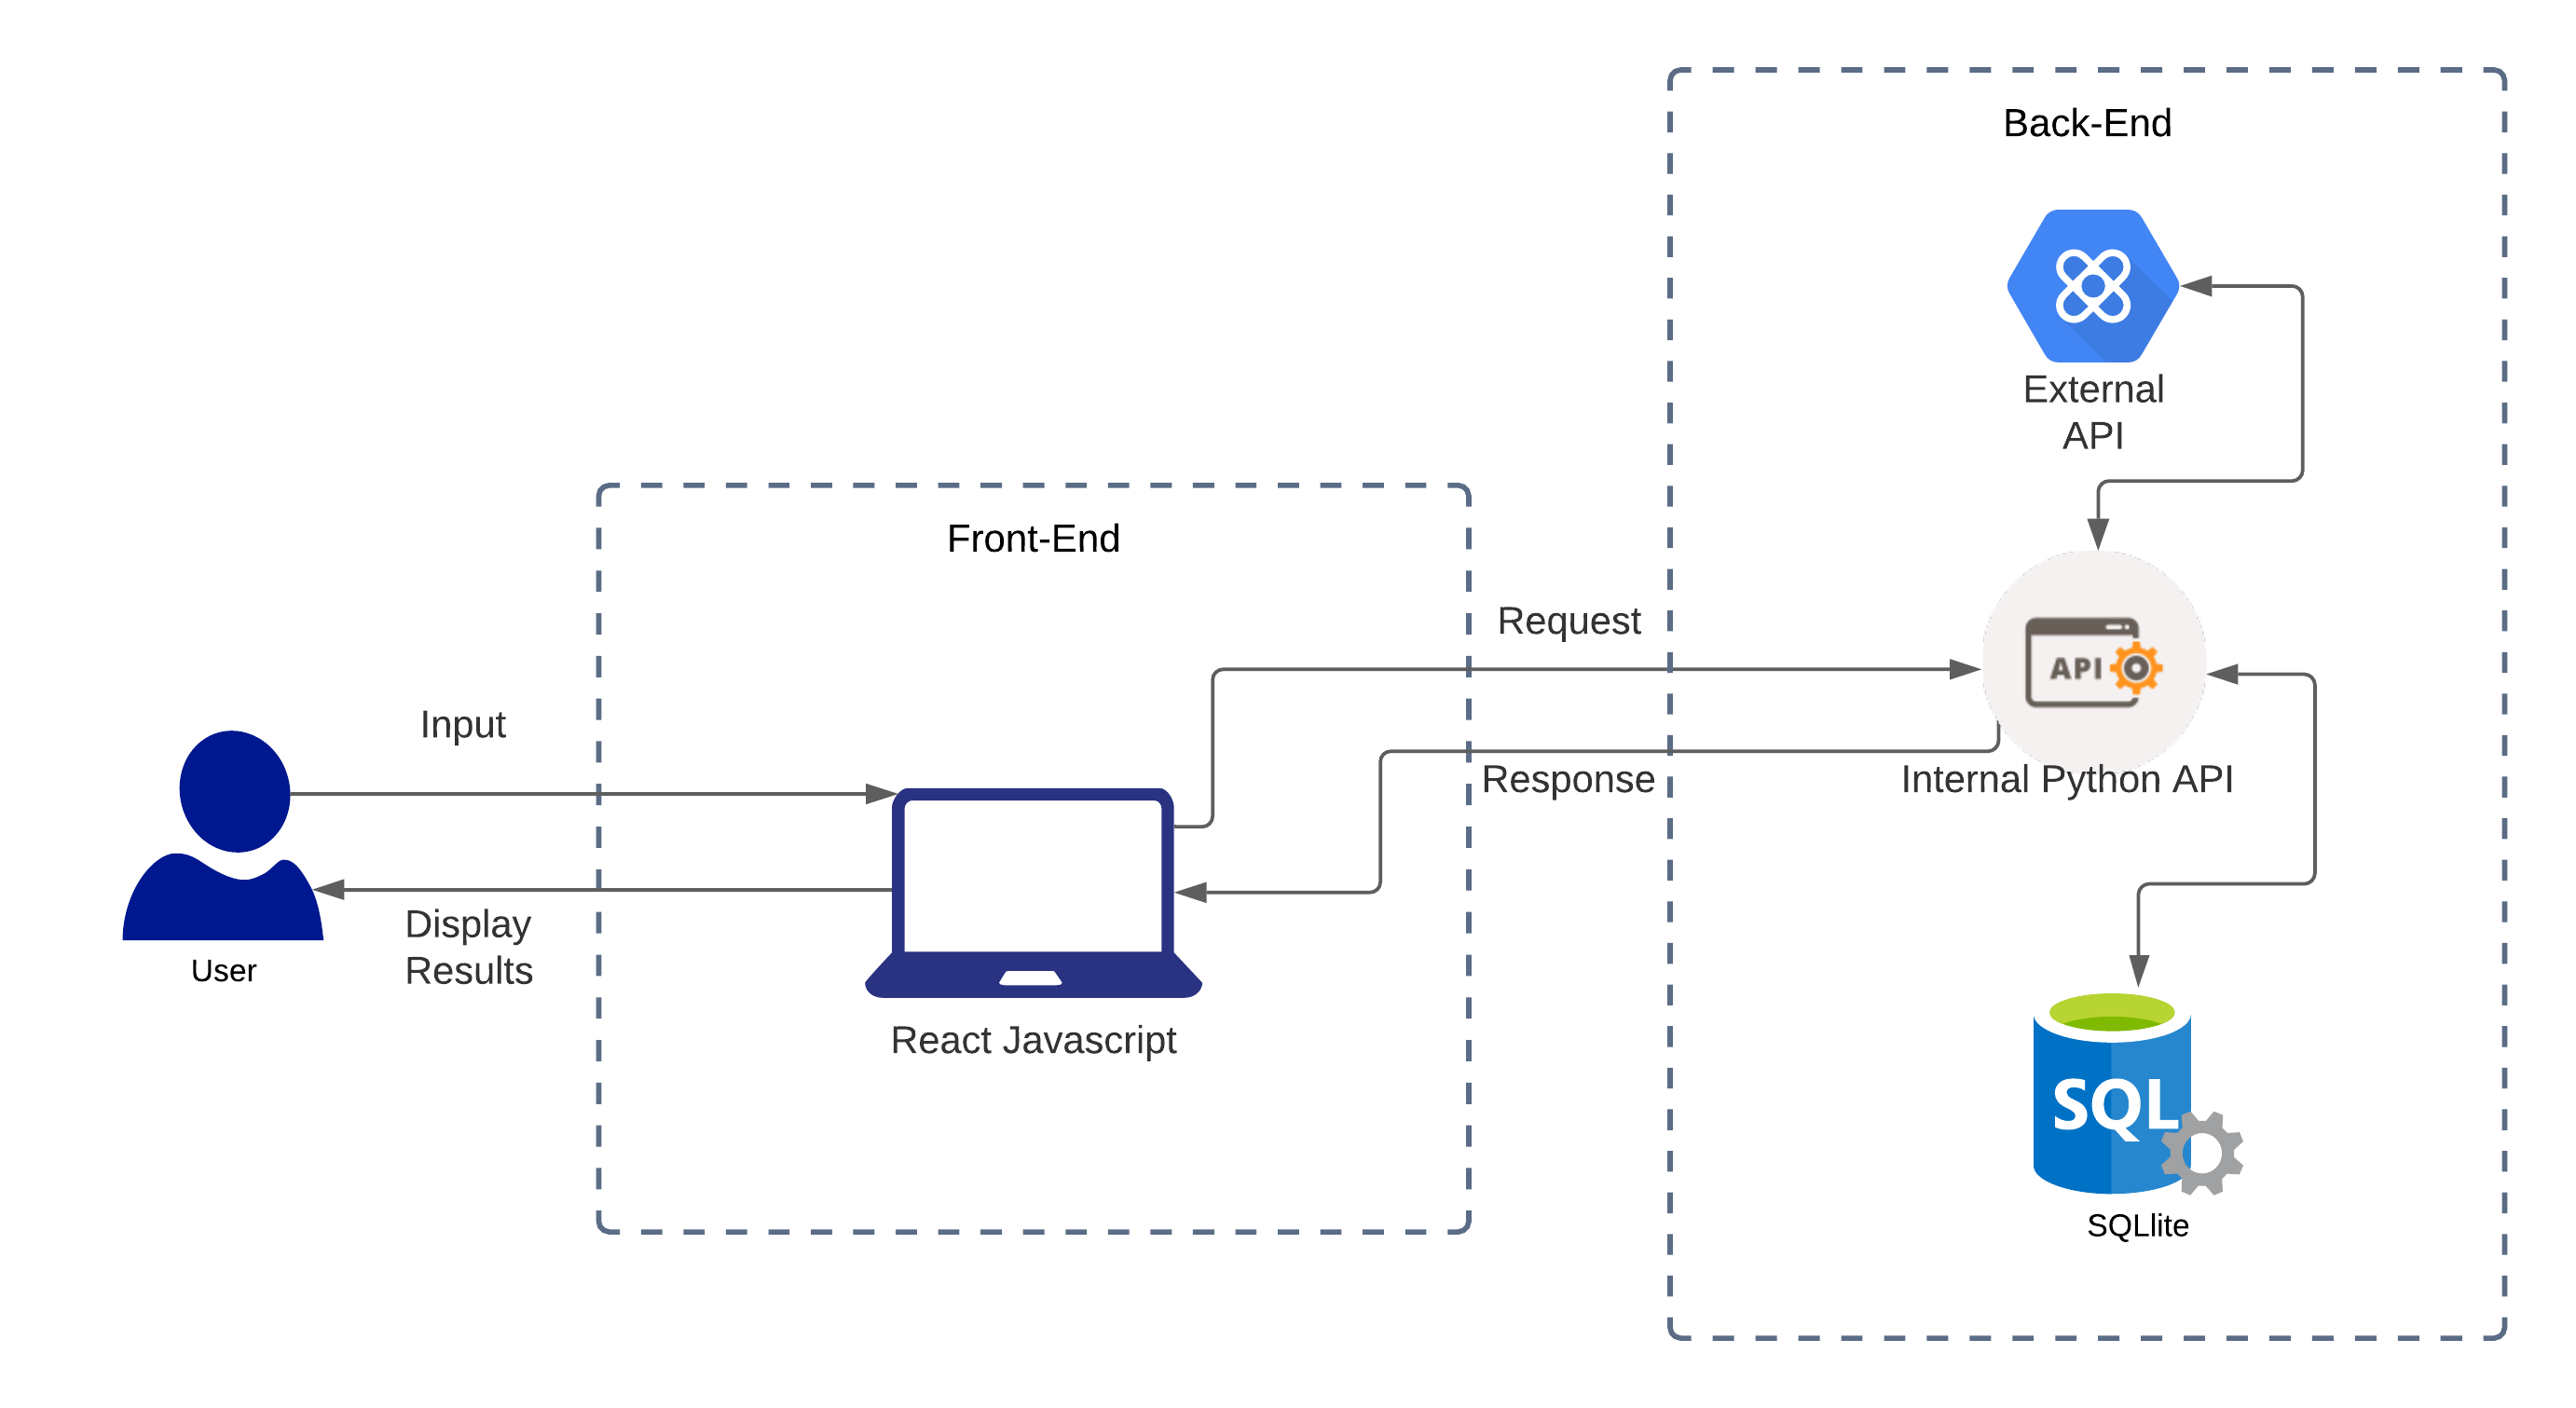
\includegraphics[scale = .7]{./5_architecture/Architecture User.png}
    \caption{Simvestr - User Interaction Diagram}
    \label{fig:Simvestr - User Interaction Diagram}
\end{figure}

\subsection{Database Structure}
Figure \ref{fig:DBMS} shows a preliminary database structure for storing relevant information in the database. To facilitate the delivery of all the functional and non-functional requirements as part of this proposal, the database will be composed of five tables; User, Portfolio, Transaction, PortfolioPrice, Watchlist, and Stock. While this may be subject to modification, we believe this database structure will scale best and allow us to add additional features within minimal schema changes.

\begin{figure}[htp]
    \centering
    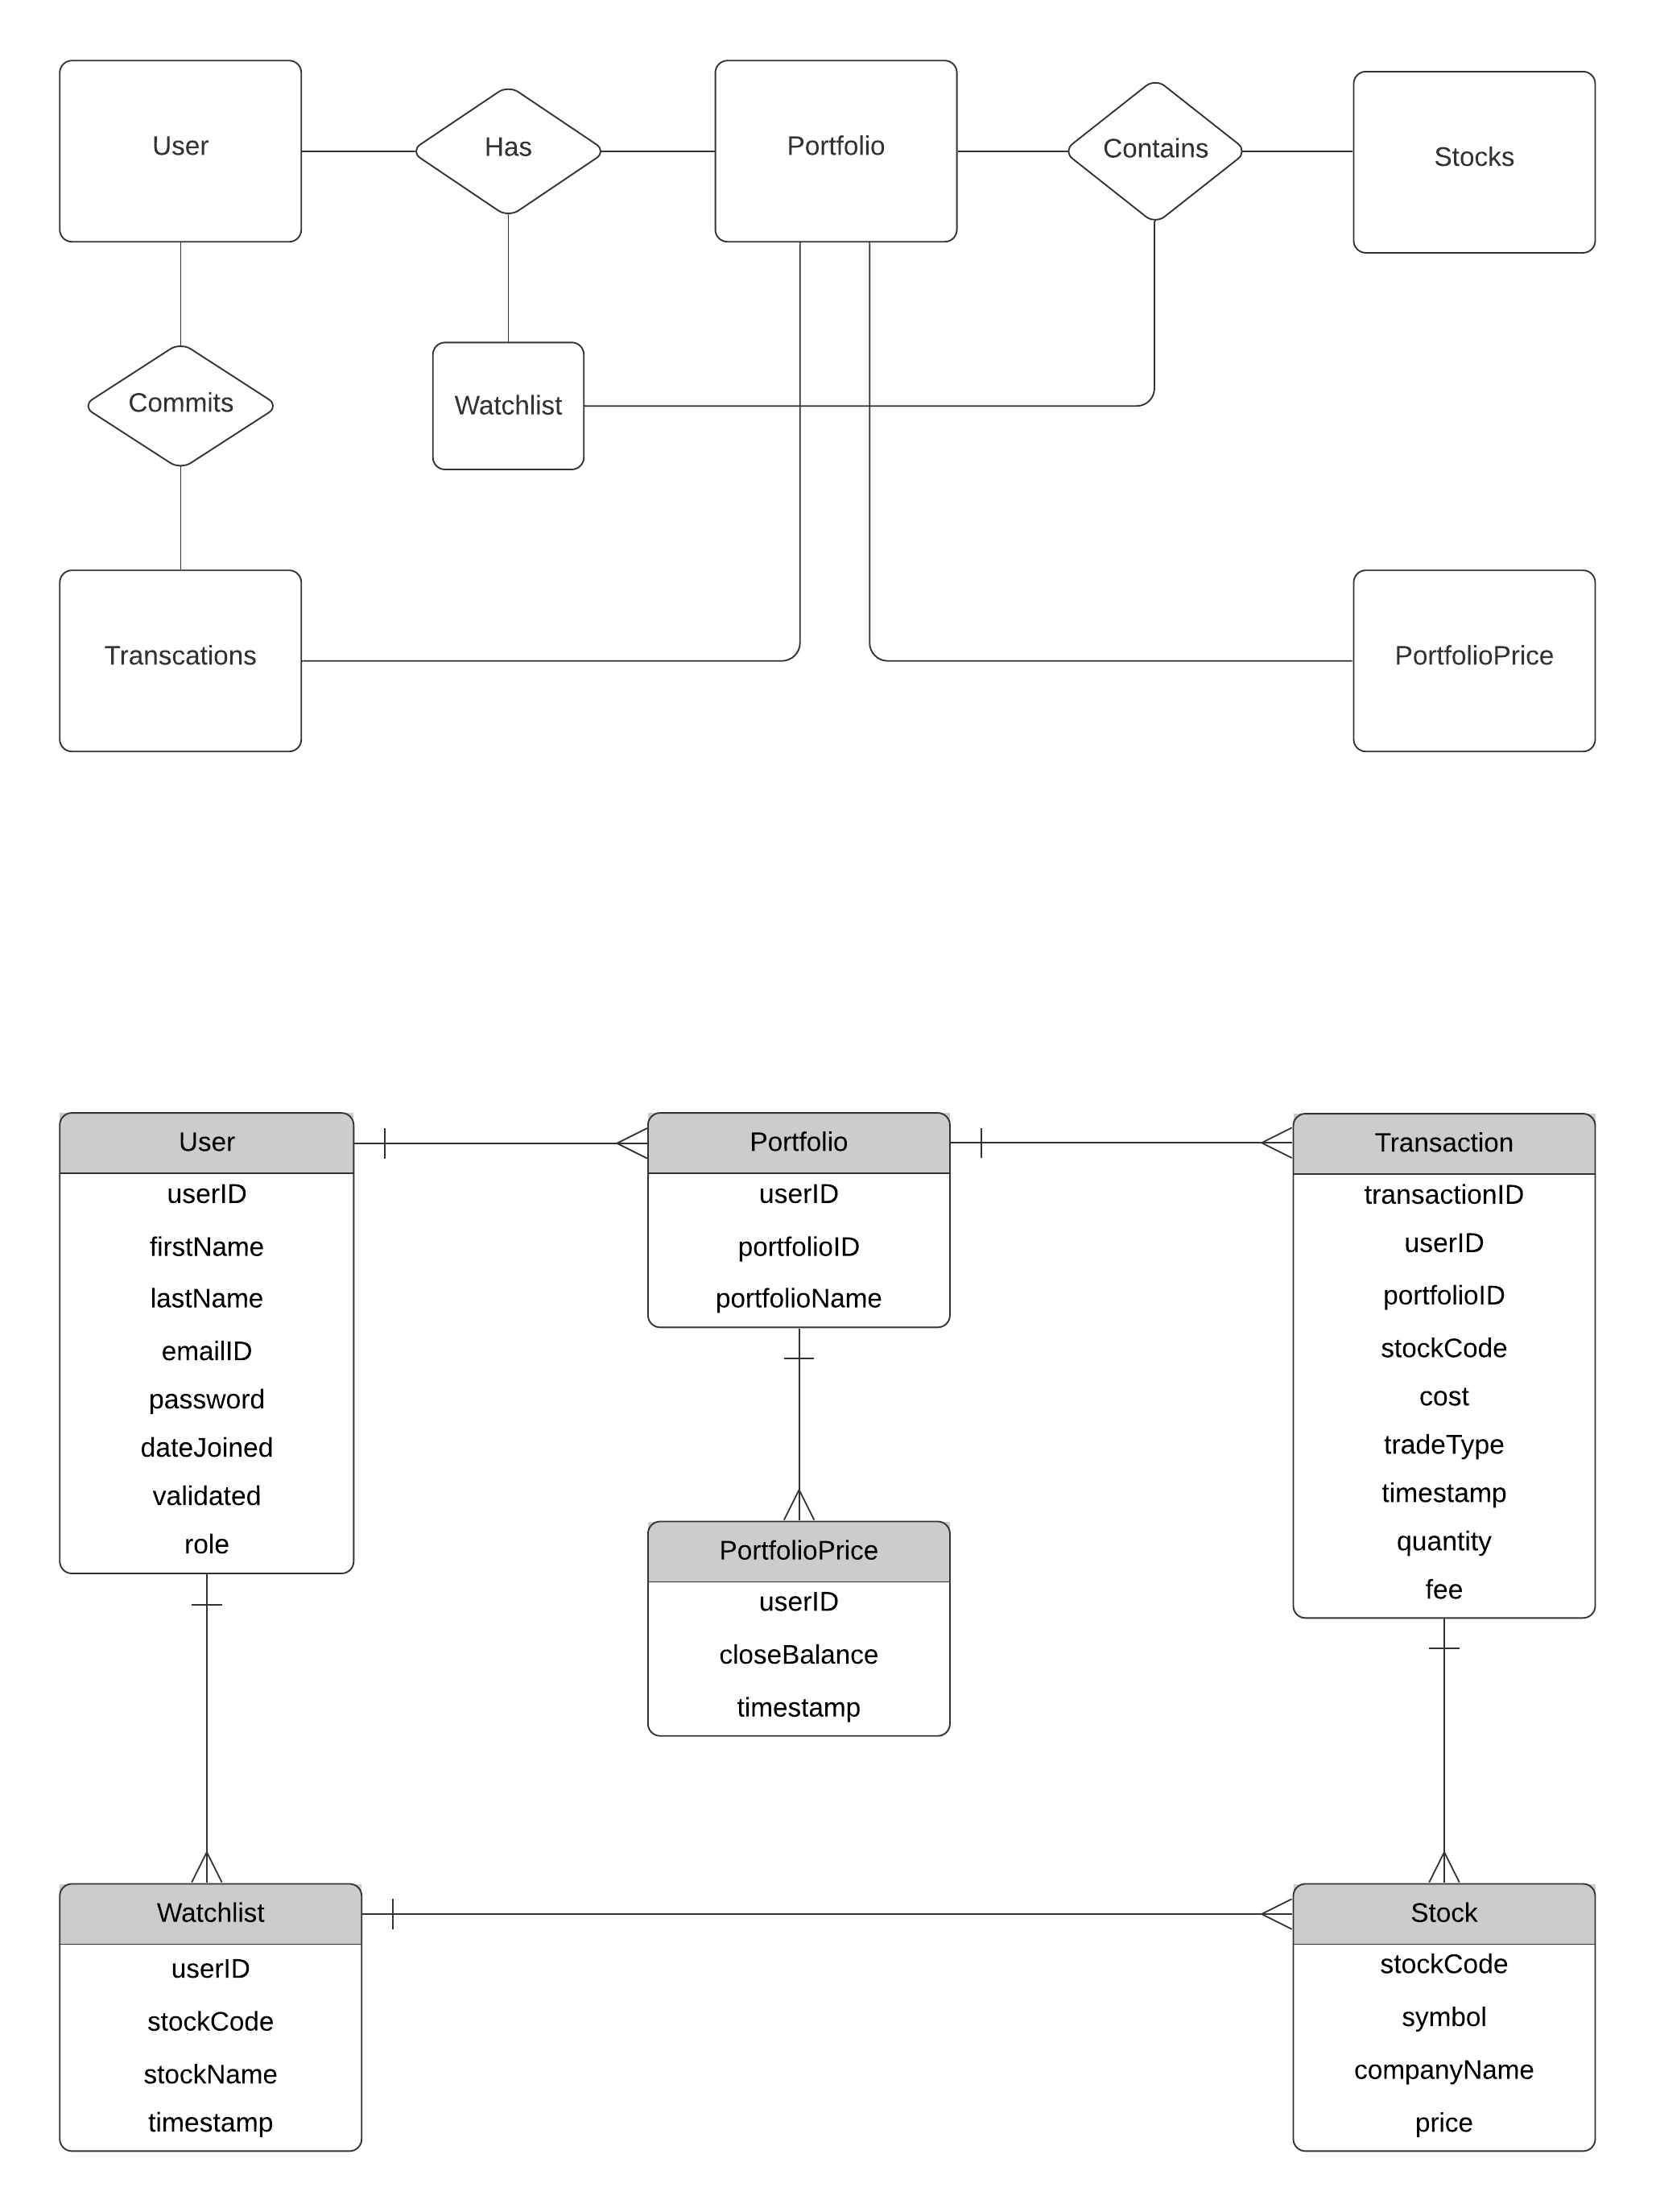
\includegraphics[scale = .8]{./5_architecture/DBMS ER diagram.png}
    \caption{Simvestr - DBMS ER Diagram}
    \label{fig:DBMS}
\end{figure}
